
\section*{Exemplo 1 Página 883}

\begin{center}
    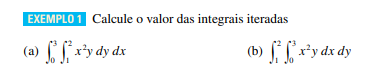
\includegraphics[scale=1.25]{enunciado.png}
\end{center}

\subsection*{(a)}

\begin{equation}
    \int_{x=0}^{x=3} \int_{y=1}^{y=2} x^2y \, dy \, dx
\end{equation}

Começamos integrando a integral "de dentro" $dy$:

\begin{equation}
    \int_{y=1}^{y=2} x^2y \, dy
\end{equation}

Note que, do ponto de vista de $y$, o termo $x^2$ é uma constante.

\begin{equation}
    \int_{y=1}^{y=2} x^2y \, dy =
    x^2\int_{y=1}^{y=2} y \, dy =
    x^2 \left[\frac{y^2}{2}\right]_{y=1}^{y=2} =
    x^2 \left[\frac{2^2}{2} - \frac{1^2}{2}\right] =
    x^2 \frac{3}{2}
\end{equation}

Assim, encontramos o valor da integral "de dentro".

\begin{equation}
    \int_{y=1}^{y=2} x^2y \, dy = \frac{3}{2} x^2
\end{equation}

Substituindo (4) em (1), temos

\begin{equation}
    \int_{x=0}^{x=3} \frac{3}{2} x^2  \, dx
\end{equation}

Primitivando (5), obtemos

\begin{equation}
    \frac{3}{2} \left[\frac{x^3}{3}\right]_{x=0}^{x=3} = 
    \frac{3}{2} \left[\frac{3^3}{3} - \frac{0^3}{3}\right] = 
    \frac{27}{2}
\end{equation}

Finalmente,

\[ \boxed{\int_{x=0}^{x=3} \int_{y=1}^{y=2} x^2y \, dy \, dx = \frac{27}{2}}  \]

\subsection*{(b)}

\begin{equation}
    \int_{y=1}^{y=2} \int_{x=0}^{x=3} x^2y \, dx \, dy
\end{equation}

Começamos integrando a integral "de dentro" $dx$:

\begin{equation}
    \int_{x=0}^{x=3} x^2y \, dx
\end{equation}

Note que, do ponto de vista de $x$, o termo $y$ é uma constante.

\begin{equation}
    \int_{x=0}^{x=3} x^2y \, dx =
    y\int_{x=0}^{x=3} x^2 \, dx =
    y \left[\frac{x^3}{3}\right]_{x=0}^{x=3} =
    y \left[\frac{3^3}{3} - \frac{0^3}{3}\right] =
    9y
\end{equation}

Assim, encontramos o valor da integral "de dentro".

\begin{equation}
    \int_{x=0}^{x=3} x^2y \, dx = 9y
\end{equation}

Substituindo (10) em (7), temos

\begin{equation}
    \int_{y=1}^{y=2} 9y \, dy
\end{equation}

Primitivando (11), obtemos

\begin{equation}
    9 \left[\frac{y^2}{2}\right]_{y=1}^{y=2} = 
    9 \left[\frac{2^2}{2} - \frac{1^2}{2}\right] = 
    9 \frac{3}{2} = \frac{27}{2}
\end{equation}

Finalmente,

\[ \boxed{\int_{y=1}^{y=2} \int_{x=0}^{x=3} x^2y \, dx \, dy = \frac{27}{2}}  \]




